\documentclass{scrartcl}
\usepackage{physics}   % Matrixes and Dirac-notation
\usepackage{amsmath}   % Binear equations
\usepackage{booktabs}  % Tabs
\usepackage{graphicx}  % Pictures/figures
\usepackage{listings}  % Source code
\usepackage{color}     % Colors
\usepackage{mdframed}  % Frames

\definecolor{dkgreen}{rgb}{0,0.6,0}
\definecolor{gray}{rgb}{0.5,0.5,0.5}
\definecolor{mauve}{rgb}{0.58,0,0.82}

%Defining source code
\lstset{frame=tb,
  language=Python,
  aboveskip=3mm,
  belowskip=3mm,
  showstringspaces=false,
  columns=flexible,
  basicstyle={\small\ttfamily},
  numbers=none,
  numberstyle=\tiny\color{gray},
  keywordstyle=\color{blue},
  commentstyle=\color{dkgreen},
  stringstyle=\color{mauve},
  breaklines=true,
  breakatwhitespace=true,
  tabsize=3
}
\makeatletter
\renewcommand*\env@matrix[1][*\c@MaxMatrixCols c]{%
  \hskip -\arraycolsep
  \let\@ifnextchar\new@ifnextchar
  \array{#1}}
\makeatother
\begin{document}
\begin{titlepage}
	\centering
	{\scshape\LARGE $\star\star\star$  \par}
	\vspace{4cm}
	{\scshape\huge FYS3110 - Quantum Mechanics  \par}
	\vspace{1cm}
	{\scshape\Large Oblig 03\par}
	\vspace{2cm}
	{\Large\itshape Even Marius Nordhagen\par}
	\vfill
	{\large \today\par}
\end{titlepage}

\section{Introduction}
Motivate the reader
Very often we are ending with a differential equation after solving a mathematical problem, for example Poisson's equation from electromagnetism. --I may should put a little historical review here--. Therefore they made some good analytical methods for solving this kind of equations, but what do we do if we need to solve this numerical? 

\section*{a)}
I will in this exercise find a matrix-representation of the Hamiltonian. This could be done for a general $n$ (I have done it numerical, see exercise $c)$), but here I will find the $4\times 4$ matrix just to spare some space. Then we have
$$\hat{H}=-g\sum_{i=0}^2\bigg(\ket{i}\bra{i+1}+\ket{i+1}\bra{i}\bigg)-V\ket{0}\bra{0}$$
$$=-g\bigg(\ket{0}\bra{1}+\ket{1}\bra{0}+\ket{1}\bra{2}
   +\ket{2}\bra{1}+\ket{2}\bra{3}+\ket{3}\bra{2}\bigg)-V\ket{0}\bra{0}$$
$$=-g\Bigg(\mqty(0&1&0&0\\0&0&0&0\\0&0&0&0\\0&0&0&0)
          +\mqty(0&0&0&0\\1&0&0&0\\0&0&0&0\\0&0&0&0)
          +\mqty(0&0&0&0\\0&0&1&0\\0&0&0&0\\0&0&0&0)
          +\mqty(0&0&0&0\\0&0&0&0\\0&1&0&0\\0&0&0&0)$$
        $$+\mqty(0&0&0&0\\0&0&0&0\\0&0&0&1\\0&0&0&0)
          +\mqty(0&0&0&0\\0&0&0&0\\0&0&0&0\\0&0&1&0)\Bigg)
          -V\mqty(1&0&0&0\\0&0&0&0\\0&0&0&0\\0&0&0&0)$$
$$\underline{\hat{H}=-q\mqty(0&1&0&0\\1&0&1&0\\0&1&0&1\\0&0&1&0)-V\mqty(1&0&0&0\\0&0&0&0\\0&0&0&0\\0&0&0&0)}$$
This is as we expect, the outer products give matrices, and we and up with to terms. In general a Hamiltonian consists of a kinetic energy term and a potential term, so the expression found above matches with this.

\section*{b)}
Here we shall find a representation for the position operator. We already know that it should have the atom indexes as eigenvalues, and the basis should be the same as in the previous exercise. We obtain
$$\hat{X}\ket{0}=0\ket{0}\quad\Rightarrow\quad\hat{X}\ket{i}=i\ket{i}$$
so mathematical we can write this as
$$x_{11}=0,\quad x_{22}=1,\quad ...\quad x_{ii}=(i-1)$$
\textit{NB! Notice that this is the mathematical implementation, numerical we will shift the indexes, so we will have $x_{ii}=i$}\par\vspace{3mm}
Therefore the matrix-representation for the position operator is
$$\hat{X}=\mqty(0&0&0&0\\0&1&0&0\\0&0&2&0\\0&0&0&3)$$
when $n=4$

\section*{c)}
When we are measuring energy, the only results we can have is the eigenvalues of $\hat{H}$. Therefore the lowest energy we can measure is the lowest (the first) eigenvalue, which has value -4.25. The energy diagram looks like this (\textit{see Figure 1}):
\begin{figure}[!htbp]
\centering
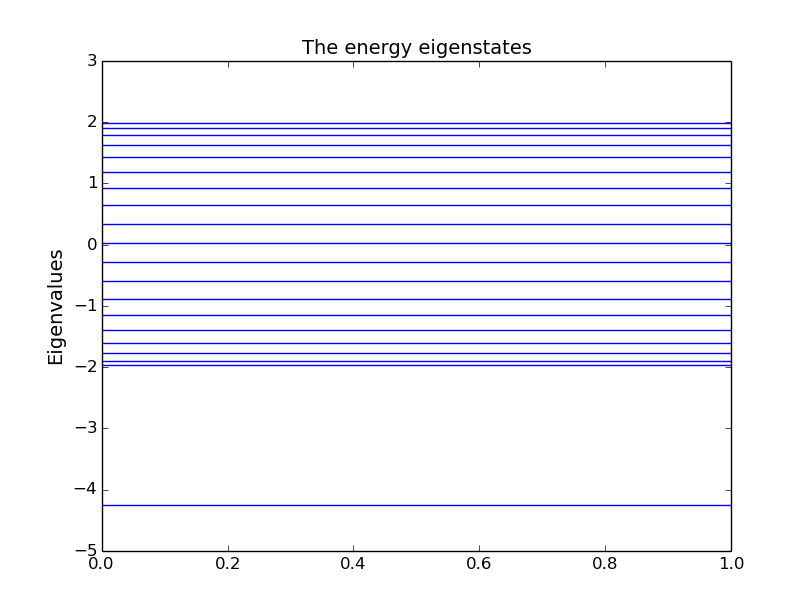
\includegraphics[width=110mm]{oblig3_1.png}
\caption{The energy eigenstates for $n=20$. \label{overflow}}
\end{figure}
\textit{I have calculated this numerical in Python, please see the appendix in the back of this assignment to find the code attachment.}

\section*{d)}
The Born rule states that
$$P(x)=|\Psi(x)|^2$$
where $\Psi(x)=\braket{x}{\psi(x)}$. In our case, I find that
$$P_g(0)=|\braket{0}{\psi_g}|^2\cong0.9375$$
$$P_g(1)=|\braket{1}{\psi_g}|^2\cong0.0586$$
Where $P_g(i)$ is the probability to find the electron by atom $i$ in the ground state. I have done the calculations numerical.

\section*{e)}
We know that the expectation value for position is given by
$$\langle x\rangle_g=\mel{\psi_g}{\hat{X}}{\psi_g}$$
where $\psi_g$ is the ground state. We can split this up to two inner products:
$$\braket{\psi_g}{\braket{\hat{X}}{\psi_g}}$$
or just
$$a=\braket{\hat{X}}{\psi_g},\quad\langle x\rangle_g=\braket{\psi_g}{a}$$
I have implemented this in my program, and got that the
$$\underline{\langle x\rangle\approx\frac{2}{3}}$$
Physical this is the place between atom 0 and atom 1, but note: There is not possible to measure this value! The electron will always be bound to a specific atom, and the expectation value is just a average over all the possible states.

\section*{f)}
In this exercise I will assume that the electron is attracted at atom 0 in the beginning. Then we will calculate the probability to find the electron on the same atom at a later time. First we know that atom 0 can be expressed as
$$\ket{0}=\sum_nC_n\ket{E_n}$$
The easiest way to find the probability at a later time is to use the propagator $\hat{U}$:
$$\hat{U}\ket{0}=\hat{U}\sum_nCn\ket{E_n}=C_ne^(-iE_nt/\hbar)\ket{E_n}$$
So the probability should be
$$P(t,0)=\sum_{n=1}^{N-1} C_ne^(-iE_nt/\hbar)\ket{E_n}$$
When I do this numerical, I get this plot:
\begin{figure}[!htbp]
\centering
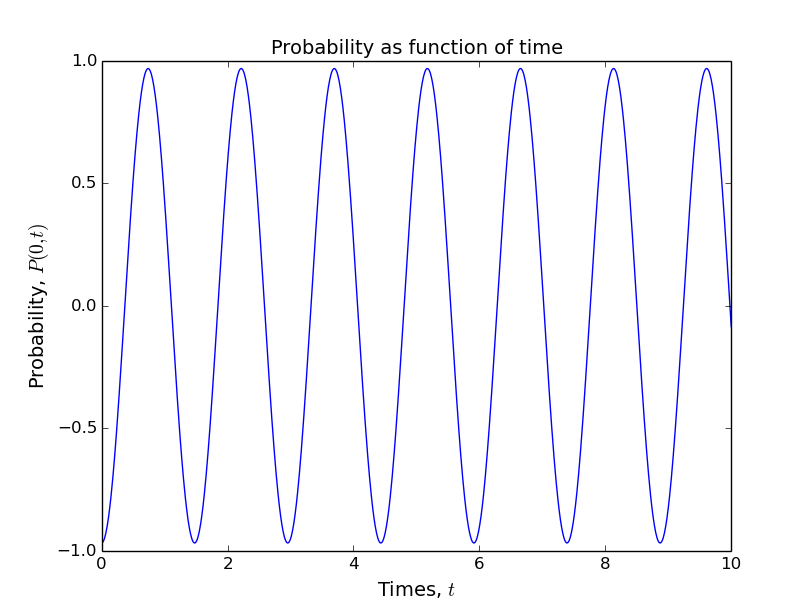
\includegraphics[width=110mm]{oblig3_2.png}
\caption{The energy eigenstates for $n=20$. \label{overflow}}
\end{figure}\par\vspace{3mm}
I know this is not the right solution, the real solution should not be harmonic. I guess is something wrong with my analytical expression. 

\section*{Code attachment}
Here is the code that I have used in this problem set:
\lstinputlisting[language=Python]{oblig3.py}
Right now this program gives the print:
\begin{lstlisting}
P_g(0) =  0.9375
P_g(1) =  0.05859375
The expectation value is:  0.0666666666667
\end{lstlisting}

\end{document}